\documentclass[a4paper]{article}
% 
% \usepackage[utf8]{inputenc}
% \usepackage[T1]{fontenc}
% \usepackage{textcomp}
% \usepackage[dutch]{babel}
% \usepackage{amsmath, amssymb}
% 
% 
% % figure support
% \usepackage{import}
% \usepackage{xifthen}
% \pdfminorversion=7
% \usepackage{pdfpages}
% \usepackage{transparent}
% \newcommand{\incfig}[1]{%
% 	\def\svgwidth{\columnwidth}
% 	\import{./figures/}{#1.pdf_tex}
% }
\usepackage{graphicx}
\usepackage{lscape}
\usepackage{longtable}
\usepackage{array}

\newcommand{\incg}[1]{\raisebox{-\totalheight}{\includegraphics[width=0.25\textwidth]{#1}}}

\graphicspath{ {/home/kristian/Documents/Shkolla/Matematike/cards/} }
\pdfsuppresswarningpagegroup=1


\title{Poker \\ një prezantim me probabilitetin e duarve të pokerit.}
\author{Kristian Blido}
\date{15, Shkurt 2021}
\begin{document}
	\maketitle
	\section* {Cfarë është pokeri?}
	Pokeri eshte nje loje qe luhet me letra, ku kombinimi me i larte i letrave fiton. Loja ka ekonomine e saj dhe lojtari ka si qellim te fitoje sa me shume monedha. Duart e pokerit perbehen nga 2 letra ne dore dhe 5 ne fushe, por vetem 5 me te mirat e gjithsecilit merren ne shqyrtim.
	\section* {Letrat në Poker}
	Letrat ne poker jane pako standarde prej 52 copesh. ato perfshijne radhitjen si me poshte:
	
	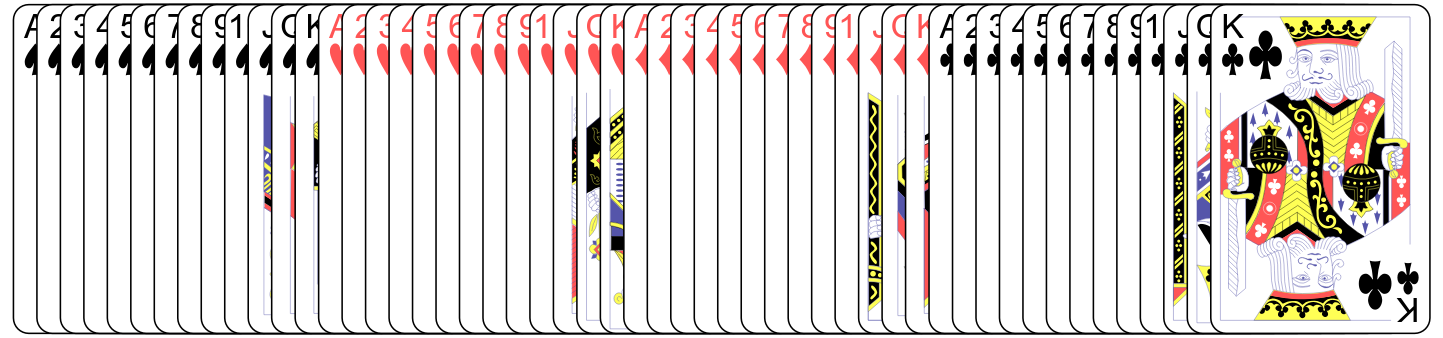
\includegraphics[width=\textwidth]{pack}
	\section*{Vlerat e letrave}
Vlerat individuale te letrave vijne duke u rritur nga e majta ne te djathte ne figuren me siper. Per sa i perket vlerave te kombinimeve, ato vleresohen sipas probabilitetit te shfaqjes se tyre:
% \begin{landscape}
	
\begin{longtable}[c]{|m{0.1\textwidth}|m{0.2\textwidth}| m{0.25\textwidth} |m{0.25\textwidth}| m{0.2\textwidth}|}
	% \begin{center}
	% \begin{tabular}{|c|c| p{5cm} |c| p{2cm}|}
	\hline	
	Vlera & Emertimi & Pershkrimi & Shembull & Probabiliteti \\
		\hline
		\hline
		\endfirsthead

			1 
		    & Straight Flush 
		    & 5 letra te njepasnjeshme me te njejten shenje. 
		    & \incg{staightflush}
			& 0.00001539 \\
			\hline
			2
			& 4 te njellojta
			& 4 letra me te njejtin numer.
			& \incg{4oak}
			& 0.00024010 \\
			\hline
			3
			& Full house
			& 3 letra me te njejtin numer dhe 3 te tjera te njllojta.
			& \incg{fullhouse}
			& 0.00144058 \\
			\hline
			4
			& Flush
			& 5 letra me te njejten shenje.
			& \incg{flush}
			& 0.00196540 \\
			\hline
			5
			& Staright
			& 5 letra te njepasnjeshme.
			& \incg{straight}
			& 0.00392465 \\
			\hline
			6
			& 3 te njellojta
			& 3 letra me te njejtin numer.
			& \incg{3oak}
			& 0.02112845 \\
			\hline
			7
			& 2 cift
			& 2 dyshe letrash me numer te njejte.
			& \incg{2pair}
			& 0.04753902 \\
			\hline
			8
			& Cift
			& nje cift letrash me numer te njejte.
			& \incg{pair}
			& 0.42256903 \\
			\hline
			9
			& Leter e larte
			& leter teke
			& \incg{high_card}
			& 0.50117739 \\
			\hline


	% \end{tabular}
	% \label{tab:label}
	% \caption{vlera e letrave}
	% \end{center}
\end{longtable}

\section* {Llogaritja e probabiliteteve}
\subsection*{Mundesi gjithsej}
Per te llogaritur probabilitetet e secils dore, duhet fillimisht te shohim sa duar mund te jene gjithesej. Nga nje pako me 52 letra zgjidhen rastesisht 5. Numri total i seteve prej 5 letrash jepet nga formula: \[
	C^{5}_{52} = \frac{52!}{5! \cdot \left( 52-5 \right)! } = 2598960
\]
\subsection*{Staright Flush}
Ne radhitjen standarde te letrave: 2, 3, 4, 5, 6, 7, 8, 9, 10, J, Q, K, A. Nje set prej 5 letrash te njepasnjeshme mund te kete fillim tek 2, 3, 4, 5, 6, 7, 8, 9, 10, A. Kjo ben qe mundesite per duar "Striaght Flush" te llogariten sipas mundesive per letren fillesate dhe shenjen e letres, pekatesisht: \[
	C^{1}_{10}\cdot C^{1}_{4}=10\cdot 4=40
\] 
Gjithesej jane 40 duar me vleren "straight flush".
Probabiliteti eshte mundesite per kete dore pjestuar me mundesite gjithesej: \[
\frac{40}{2598960}\approx 0.00001539
\]
\subsection*{4 te njellojta}
Jane vetem 13 mundesi per 4 letra te njellojta, pasi secili numer perseritet 4 here ne nje pako me 3 shenja te ndryshme. Megjithate, duar qe kane vleren "4 te njellojta" jane: \[
	C_{13}^{1} \cdot  C_{48}^{1} = 13 \cdot 48 = 624
\] 
13 mundesi per katershen e letrave, dhe 52-4 per letren e 5te.
Probabiliteti: \[
\frac{624}{2598960}\approx 0.00024010
\]
\subsection*{Full House}
Doren "Full House" mund ta imagjinojme si dy sete, njeri me 3 letra te njejta dhe tjetri me 2 te njejta. Kjo ben qe mundesite per setin e pare te caktohen sipas numrit dhe shenjes ashtu si dhe per setin e dyte. Seti i pare ka 13 mundesi per numrin, dhe 4 mundesi per shenjen, nga te cialt vetem 3 do zgjidhen: \[
	C_{13}^{1} \cdot  C_{4}^{3}
\] 
Njelloj edhe per setin e dyte kemi $13-1$ mundesi per numrin dhe 4 mundesi per shenjen nga te cilat do zgjidhen vetem 2: \[
	C_{12}^{1} \cdot  C_{4}^{2}
\]
 Mundesite per komplet setin prej 5 letrash jane:
$$	C_{13}^{1} \cdot  C_{4}^{3} \cdot C_{12}^{1} \cdot  C_{4}^{2}$$
$$	13\cdot 4 \cdot 12\cdot 6 = 3744 $$
Ideja per probabilitetin eshte e njellojte ne tere rastet, qe tani e tutje referoju tabeles per vlerat e sakte te probabilitetve.
\subsection*{Flush}
Per te arritur "Flush" na duhen 5 letra me shenje te njejte dhe numri nuk na intereson, ne gjuhe matematike kjo shprehet si: \[
	C_{4}^{1}\cdot C_{13}^{5}
\]
Megjithate kjo formule perfshin edhe llojet "Staright Flush", te numeruar me larte. Nje dore e atille ka vlere te ndryshme nga "Flush" i thjeshte dhe duhen hequr nga numri: \[
	C_{4}^{1}\cdot C_{13}^{5} - 40 = 4\cdot 1287 -40 = 5108
\]
\subsection*{Straight}
Per te arritur "Straight" duhet nje leter fillimi qe sic thame me lart, jane 10 mundesi. Cdo leter sa kohe ka numrin e pershtatshem, mund te kete cdo shenje. Keshtu, mundesite per letren e fillimit jane $C_{10}^{1}\cdot C_{4}^{1}$ kjo llogarit mundesite per numrin e letres se pare te radhitjes se njepasnjeshme (kjo leter mund te kete pozicionin e fundit ne dore, por per lehtesi llogaritje hamendesojme qe eshte e para edhe ne dore). Pasi kemi "zgjedhur" letren e pare te setit, 4 letrat e tjera kane secila vetem 1 mundesi per numrin por 4 mundesi secila per shenjen: \[
	C^{1}_{10} \cdot (C^{1}_{4})^{5}-40=10\cdot 1024-40=10200
\] 
Heqim 40 per te njejten arsye si me larte, ato jane 40 duart e numeruara tek rasti "Staright Flush".
\subsection*{3 te njellojta}
Kjo dore permban 3 letra me te njejtin numer dhe 2 te tjera te rastesishte. Si ne rastin "Full House" e mendojme doren si dy sete: 3 letra me te njejtin numer, dhe 2 letra tjera.
Mundesite per 3 letra me te njejtin numer caktohen nga numri i letres $C_{13}^{1}$ dhe nga shenja e seciles prej tre letrave $C_{4}^{3}$. Mundesite e dy letrave tjera caktohen nga numri i seciles leter dhe nga shenja e seciles $C_{12}^{2}\cdot (C_{4}^{1})^2$. \[
C_{13}^{1}\cdot C_{4}^{3}\cdot C_{12}^{2}\cdot (C_{4}^{1})^2=13\cdot 4\cdot 66 \cdot 16 =54912
\]
\subsection*{2 dyshe}
Mundesite per te pasur 2 dyshe dhe nje leter te 5te te rastesishme te ndryshme nga te parat caktohet nga prodhimi i mundesive per numrin e dy te parave, shenjen e dy te parave, numrin e dy te dytave, shenjen e dy te dytave dhe mundesite per letren e fundit. Numri i ciftit te pare dhe te dyte caktohet nga $C_{13}^{2}$ dhe ngjyra e secilit cift nga $C_{4}^{2}$. Letra e fundit ka mundesi $C_{44}^{1}$. \[
	C_{13}^{2}\cdot (C_{4}^{2})^{2}\cdot C_{44}^{1}=78\cdot \cdot 36\cdot 44=123552
\] 
\subsection*{Cift}
Ne menyre te ngjashme me rastin me larte, mundesite per nje cift jane prodhimi i mundeisve per numrin e dy letrave, shenjen e letrave, numrin e tre te tjerave dhe shenjen se seciles: \[
	C_{13}^{1}\cdot C_{4}^{2}\cdot C_{12}^{3}\cdot (C_{4}^{1})^{3}=13\cdot 6\cdot 220\cdot 64 =1098240
\] 
\subsection*{Leter e Larte}
Per te llogaritur mundesite e kesaj dore do ndjekim nje rruge tjeter. Qe te mos ndodh asnje kombinim do te thote qe nga gjithe mundesite, te perjashtojme ato qe kane kombinime, perkatesisht: \[
	C_{52}^{5} - \textrm{Shume e mundesive te gjithe kombinimeve me lart} =2598960-1296420=1302540
\] 
\end{document}
